\section{Robust Signomial Programming} \label{RSP}
Robust signomial programming (RSP) assumes that parameter uncertainties belong to an uncertainty set, and solves the design problem to find the best solution as shown in Figure \ref{block_diag}. This section introduces RSPs and derives the intractable formulation of an RSP.

\begin{figure}[h]
	\centering
	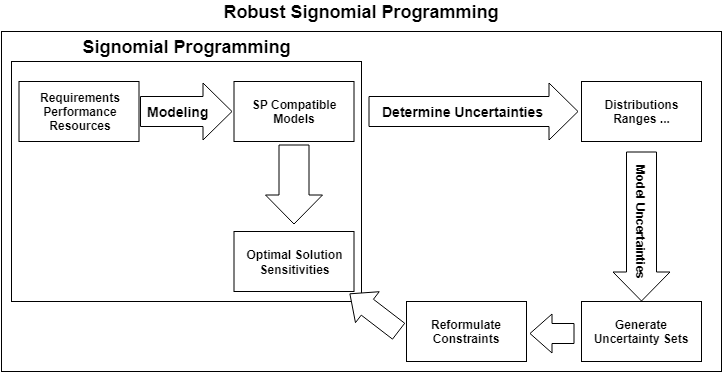
\includegraphics{figures/RSP_Diagram.png}
	\caption{A block diagram showing the difference between the design process using an SP and an RSP.}
	\label{block_diag}
\end{figure}

An SP in its \textbf{exponential form} is as follows:

\begin{equation}
\begin{aligned}
	& \min && f_0\left(\vec{x}\right) \\
	& \text{s.t.} && \textstyle{\sum}_{k=1}^{K_i}e^{\vec{a_{ik}}\vec{x} + b_{ik}} - \textstyle{\sum}_{k=1}^{G_i}e^{\vec{c_{ik}}\vec{x} + d_{ik}} \leq 0 \quad \forall i \in 1,...,m\\
\end{aligned}
\label{SP_exponential}
\end{equation}

Let $\vec{a_{ik}}$ and $\vec{c_{ik}}$ be the $((i-1)\times m + k)^{th}$ rows of the exponents matrices $\mat{A}$ and $\mat{C}$ respectively, and $b_{ik}$ and $d_{ik}$ be the $((i-1)\times m + k)^{th}$ elements of the coefficients vectors $\vec{b}$ and $\vec{d}$ respectively.

The data ($\mat{A}$, $\mat{C}$, $\vec{b}$, $\vec{d}$) is assumed uncertain and living in an uncertainty set $\mathcal{U}$, where $\mathcal{U}$ is parametrized affinely by a perturbation vector $\vec{\zeta}$ as follows:

\begin{equation}
\mathcal{U} = \left\{\left[\mat{A};\mat{C};\vec{b};\vec{d}\right] = \left[\mat{A}^0;\mat{C}^0;\vec{b}^0\;\vec{d}^0 \right] + \textstyle{\sum_{l=1}^{L}\zeta_l\left[\mat{A}^l;\mat{C}^l;\vec{b}^l; \vec{d}^l\right]}\right\}
\label{Data}
\end{equation}
where $\mat{A}^0$, $\mat{C}^0$, $\vec{b}^0$, and $\vec{d}^0$ are the nominal exponents and coefficients, $\left\{\mat{A}^l\right\}_{l=1}^{L}$, $\left\{\mat{C}^l\right\}_{l=1}^{L}$, $\left\{\vec{b}^l\right\}_{l=1}^{L}$, and $\left\{\vec{d}^l\right\}_{l=1}^{L}$ are the basic shifts of the exponents and coefficients, and $\zeta_l$ is the $l^{th}$ component of $\vec{\zeta}$ belonging to a conic perturbation set $\mathcal{Z} \in \mathbb{R}^L$ paramaterized by $\mat{F},\,\mat{G},\,\vec{h}$ and $\textbf{K}$ such that
\begin{equation}
\mathcal{Z} = \left\{ \vec{\zeta} \in \mathbb{R}^L: \exists \vec{u} \in \mathbb{R}^k:\mat{F}\vec{\zeta} + \mat{G}\vec{u} + \vec{h} \in \textbf{K} \right\}
\label{perturbation_set}
\end{equation}
where $\mathbf{K}$ is a regular cone in $\mathbb{R}^N$ with a non-empty interior if it is not polyhedral, $\mat{F} \in \mathbb{R}^{N \times L}$, $\mat{G} \in \mathbb{R}^{N \times k}$, and $\vec{h} \in \mathbb{R}^{N}$. 

As mentioned earlier, there should exist a formulation immune to uncertainty in the system's data. Accordingly, the robust counterpart of the uncertain signomial program in \eqref{SP_exponential} is:
\begin{equation}
\begin{aligned}
& \min && f_0\left(\vec{x}\right) \\
& \text{ s.t.} && \textstyle{\sum}_{k=1}^{K_i}e^{\vec{a_{ik}}\left(\zeta\right)\vec{x} + b_{ik}\left(\zeta\right)} - \textstyle{\sum}_{k=1}^{G_i}e^{\vec{c_{ik}}\left(\zeta\right)\vec{x} + d_{ik}\left(\zeta\right)} \leq 0 \quad \forall i \in 1,...,m && \forall \vec{\zeta} \in \mathcal{Z}\\
\end{aligned}
\label{SP_counterparts}
\end{equation}
These constraints state that the robust optimal solution should be feasible for all possible realizations of the perturbation vector $\vec{\zeta}$. However, the above is a semi-infinite optimization problem, i.e. an optimization problem with finite number of variables and infinite number of constraints. Such a problem is intractable using current solvers and so an equivalent finite set of constraints is usually derived:
\begin{equation}
\begin{aligned}
& \min &&f_0\left(\vec{x}\right)\\
& \text{subject to} &&\max_{\vec{\zeta} \in \mathcal{Z}} \left\{\textstyle{\sum}_{k=1}^{K_i}e^{\vec{a_{ik}}\left(\zeta\right)\vec{x} + b_{ik}\left(\zeta\right)} - \textstyle{\sum}_{k=1}^{G_i}e^{\vec{c_{ik}}\left(\zeta\right)\vec{x} + d_{ik}\left(\zeta\right)}\right\} &&\leq 1 &&\forall i \in 1,...,m\\
\end{aligned}
\label{SP_counterparts_finite}
\end{equation}

The optimization problem in \eqref{SP_counterparts_finite} is intractable. In the following sections, a heuristic approach to solving RSPs approximately as a sequential RGP will be presented. As our approach is based on Robust Geometric Programming, a brief review of the subject will follow based on \cite{Saab2018}. 